\section{Where a loop's gain comes from}\label{sec:round1}
\begin{figure}[t]\centering
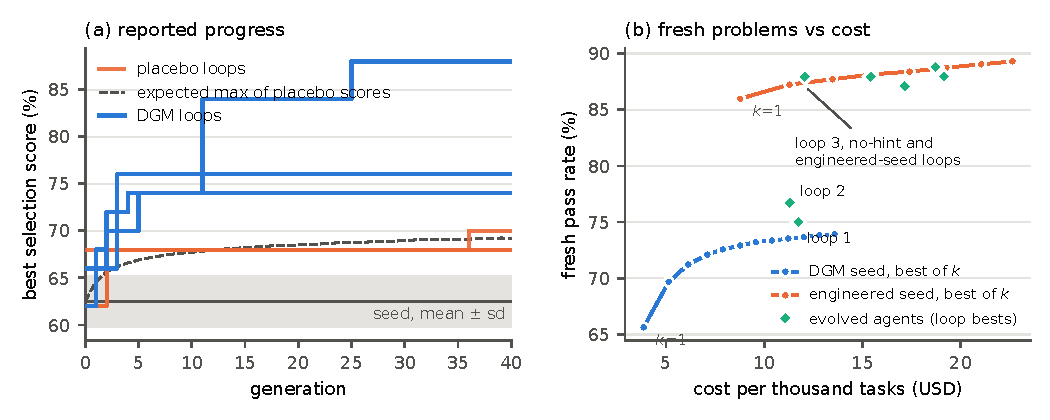
\includegraphics[width=\linewidth]{fig1.pdf}
\caption{First-round loops. (a) Best selection score by generation. Placebo loops (children are exact copies) rise to the expected
maximum of their own noisy scores (dashed); DGM loops rise above it. (b) Pass rate on $F_1$ against cost per task.
Lines: the unchanged seeds run $k$ times, submitting the first solution that passes the examples in the problem statement.
Diamonds: best agents of the loops.}\label{fig:main}
\end{figure}

\paragraph{Selection on noise.} The unchanged seed scores $\nseedDgmSmean\% \pm \nseedDgmSsd$ on $S$ over
$\nseedDgmSn$ evaluations (its own and those of placebo copies, which have identical code). The $\vhPlaceboN$ placebo
loops evaluate about 80 copies each on the full selection set and
report best scores of $\vhPlaceboMin$ to $\vhPlaceboMax\%$; the expected maximum of that many independent draws with the
seed's mean and spread is $\vhPlaceboPred\%$ (Figure~\ref{fig:main}a shows the three first-round placebo loops and the three first-round DGM loops). A loop's best
selection score therefore carries a noise term of about seven points, predictable from the rerun spread and the number of full evaluations. For the DGM
loops the selection gain exceeds the fresh gain in every loop, by about four points on average, but with each loop's
sampling error this is not significant (H2; \S\ref{sec:results2}).

\paragraph{Compute.} Evolved agents spend more per task than the seed. Rerunning the unchanged seed several times and
submitting the first solution that passes the examples in the problem statement (Table~\ref{tab:compute}) accounts for most
of the fresh gains of two of the three first-round loops at similar cost: their best agents differ from the
seed at matched cost by $\nvskLoopA$ [$\nvskLoopAlo$, $\nvskLoopAhi$] and $\nvskLoopB$ [$\nvskLoopBlo$, $\nvskLoopBhi$]
points on $F_1$. Resampling does not reproduce the third loop's gain even at twelve attempts, which still cost less
than that agent, probably because the seed fails the same problems on every attempt.

\paragraph{Repair.} The seed requests at most 4{,}096 output tokens. The task model's default reasoning often uses that
budget up on hard problems, and the agent then receives neither text nor a tool call and stops; $\nseedEmptyShare\%$ of
the seed's fresh runs end with no solution. Loop 3's best agent recovers from such empty turns by retrying with larger
budgets, nudges and fallback calls. Raising the seed's cap to 16{,}000 tokens and changing nothing else gains
$\vlvCapgain$ points [$\vlvCapgainlo$, $\vlvCapgainhi$] on all fresh problems in the final batch that re-evaluated every
loop agent together (Table~\ref{tab:loops}), where it trails loop 3's agent by $\vcapVsLoopFinAbs$ points [$\vcapVsLoopFinAbslo$,
$\vcapVsLoopFinAbshi$] at about a third of its cost per task; in the batch of the lineage ablation (\S\ref{sec:round2}) it trails by $\vcapvsloopthreeAbs$
[$\vcapvsloopthreeAbslo$, $\vcapvsloopthreeAbshi$]. The cap-only seed is an exploratory arm.

\paragraph{Other first-round results} (details in Appendix~\ref{app:round1}). Single edits proposed from the agent's
code alone gain about two points; single DGM steps gain 1.9 times as much when children that failed to compile count
as unchanged, and 2.7 times as much when those children are left out, mostly through the DGM's hand-written empty-patch prompt. Loops started from the engineered seed (a short harness that already avoids the empty-turn failure)
gain about two points on fresh problems (\nhFourCI). Under a bug in our first grader, most of the measured gain
of loops started from that harness was recovery from the bug; re-scoring the saved archives with the corrected grader
shows this without new agent runs. Under other task models, evolved agents gain most where the seed fails worst, and loop 3's agent costs
\ncostRatioRange{} times as much per task as the seed. These small first-round gains are measured against a seed reference that
pools runs from different hours (Appendix~\ref{app:round1}).

\begin{table}[t]\centering\small
\caption{The unchanged seed run $k$ times, submitting the first solution that passes the sample tests in the problem statement
($F_1$; averaged over orderings of the available runs). Cost in dollars per thousand tasks.}\label{tab:compute}
\begin{tabular}{lrrrrr}\toprule
 & $k=1$ & $k=2$ & $k=3$ & $k=6$ & $k=12$ \\ \midrule
DGM seed, pass rate & \natkDgmOne & \natkDgmTwo & \natkDgmThree & \natkDgmSix & \natkDgmTwelve \\
\quad cost & \natkDgmOneusd & \natkDgmTwousd & \natkDgmThreeusd & \natkDgmSixusd & \natkDgmTwelveusd \\ \bottomrule
\end{tabular}\end{table}
